\documentclass[1p]{elsarticle_modified}
%\bibliographystyle{elsarticle-num}

%\usepackage[colorlinks]{hyperref}
%\usepackage{abbrmath_seonhwa} %\Abb, \Ascr, \Acal ,\Abf, \Afrak
\usepackage{amsfonts}
\usepackage{amssymb}
\usepackage{amsmath}
\usepackage{amsthm}
\usepackage{scalefnt}
\usepackage{amsbsy}
\usepackage{kotex}
\usepackage{caption}
\usepackage{subfig}
\usepackage{color}
\usepackage{graphicx}
\usepackage{xcolor} %% white, black, red, green, blue, cyan, magenta, yellow
\usepackage{float}
\usepackage{setspace}
\usepackage{hyperref}

\usepackage{tikz}
\usetikzlibrary{arrows}

\usepackage{multirow}
\usepackage{array} % fixed length table
\usepackage{hhline}

%%%%%%%%%%%%%%%%%%%%%
\makeatletter
\renewcommand*\env@matrix[1][\arraystretch]{%
	\edef\arraystretch{#1}%
	\hskip -\arraycolsep
	\let\@ifnextchar\new@ifnextchar
	\array{*\c@MaxMatrixCols c}}
\makeatother %https://tex.stackexchange.com/questions/14071/how-can-i-increase-the-line-spacing-in-a-matrix
%%%%%%%%%%%%%%%

\usepackage[normalem]{ulem}

\newcommand{\msout}[1]{\ifmmode\text{\sout{\ensuremath{#1}}}\else\sout{#1}\fi}
%SOURCE: \msout is \stkout macro in https://tex.stackexchange.com/questions/20609/strikeout-in-math-mode

\newcommand{\cancel}[1]{
	\ifmmode
	{\color{red}\msout{#1}}
	\else
	{\color{red}\sout{#1}}
	\fi
}

\newcommand{\add}[1]{
	{\color{blue}\uwave{#1}}
}

\newcommand{\replace}[2]{
	\ifmmode
	{\color{red}\msout{#1}}{\color{blue}\uwave{#2}}
	\else
	{\color{red}\sout{#1}}{\color{blue}\uwave{#2}}
	\fi
}

\newcommand{\Sol}{\mathcal{S}} %segment
\newcommand{\D}{D} %diagram
\newcommand{\A}{\mathcal{A}} %arc


%%%%%%%%%%%%%%%%%%%%%%%%%%%%%5 test

\def\sl{\operatorname{\textup{SL}}(2,\Cbb)}
\def\psl{\operatorname{\textup{PSL}}(2,\Cbb)}
\def\quan{\mkern 1mu \triangleright \mkern 1mu}

\theoremstyle{definition}
\newtheorem{thm}{Theorem}[section]
\newtheorem{prop}[thm]{Proposition}
\newtheorem{lem}[thm]{Lemma}
\newtheorem{ques}[thm]{Question}
\newtheorem{cor}[thm]{Corollary}
\newtheorem{defn}[thm]{Definition}
\newtheorem{exam}[thm]{Example}
\newtheorem{rmk}[thm]{Remark}
\newtheorem{alg}[thm]{Algorithm}

\newcommand{\I}{\sqrt{-1}}
\begin{document}

%\begin{frontmatter}
%
%\title{Boundary parabolic representations of knots up to 8 crossings}
%
%%% Group authors per affiliation:
%\author{Yunhi Cho} 
%\address{Department of Mathematics, University of Seoul, Seoul, Korea}
%\ead{yhcho@uos.ac.kr}
%
%
%\author{Seonhwa Kim} %\fnref{s_kim}}
%\address{Center for Geometry and Physics, Institute for Basic Science, Pohang, 37673, Korea}
%\ead{ryeona17@ibs.re.kr}
%
%\author{Hyuk Kim}
%\address{Department of Mathematical Sciences, Seoul National University, Seoul 08826, Korea}
%\ead{hyukkim@snu.ac.kr}
%
%\author{Seokbeom Yoon}
%\address{Department of Mathematical Sciences, Seoul National University, Seoul, 08826,  Korea}
%\ead{sbyoon15@snu.ac.kr}
%
%\begin{abstract}
%We find all boundary parabolic representation of knots up to 8 crossings.
%
%\end{abstract}
%\begin{keyword}
%    \MSC[2010] 57M25 
%\end{keyword}
%
%\end{frontmatter}

%\linenumbers
%\tableofcontents
%
\newcommand\colored[1]{\textcolor{white}{\rule[-0.35ex]{0.8em}{1.4ex}}\kern-0.8em\color{red} #1}%
%\newcommand\colored[1]{\textcolor{white}{ #1}\kern-2.17ex	\textcolor{white}{ #1}\kern-1.81ex	\textcolor{white}{ #1}\kern-2.15ex\color{red}#1	}

{\Large $\underline{11a_{229}~(K11a_{229})}$}

\setlength{\tabcolsep}{10pt}
\renewcommand{\arraystretch}{1.6}
\vspace{1cm}\begin{tabular}{m{100pt}>{\centering\arraybackslash}m{274pt}}
\multirow{5}{120pt}{
	\centering
	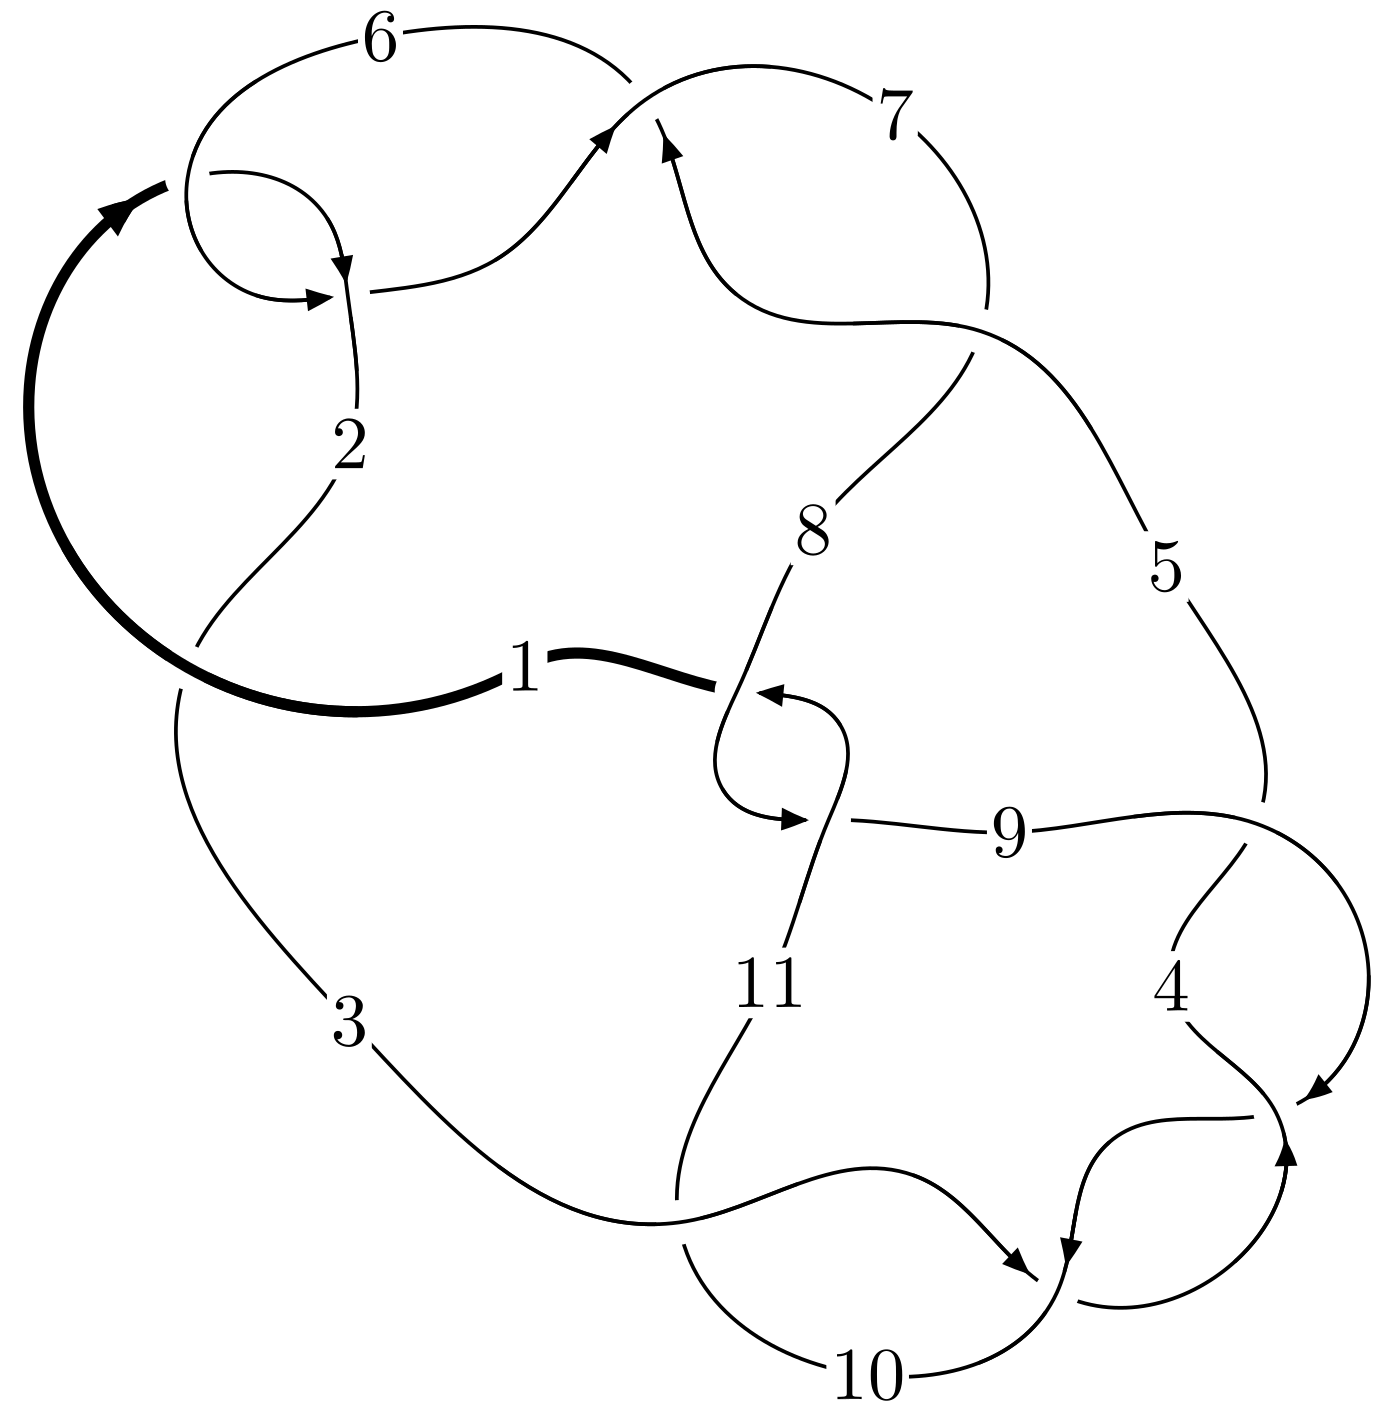
\includegraphics[width=112pt]{../../../GIT/diagram.site/Diagrams/png/478_11a_229.png}\\
\ \ \ A knot diagram\footnotemark}&
\allowdisplaybreaks
\textbf{Linearized knot diagam} \\
\cline{2-2}
 &
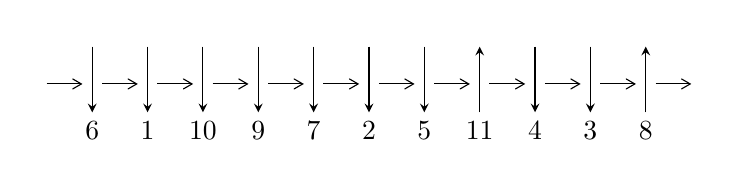
\begin{tikzpicture}[x=20pt, y=17pt]
	% nodes
	\node (C0) at (0, 0) {};
	\node (C1) at (1, 0) {};
	\node (C1U) at (1, +1) {};
	\node (C1D) at (1, -1) {6};

	\node (C2) at (2, 0) {};
	\node (C2U) at (2, +1) {};
	\node (C2D) at (2, -1) {1};

	\node (C3) at (3, 0) {};
	\node (C3U) at (3, +1) {};
	\node (C3D) at (3, -1) {10};

	\node (C4) at (4, 0) {};
	\node (C4U) at (4, +1) {};
	\node (C4D) at (4, -1) {9};

	\node (C5) at (5, 0) {};
	\node (C5U) at (5, +1) {};
	\node (C5D) at (5, -1) {7};

	\node (C6) at (6, 0) {};
	\node (C6U) at (6, +1) {};
	\node (C6D) at (6, -1) {2};

	\node (C7) at (7, 0) {};
	\node (C7U) at (7, +1) {};
	\node (C7D) at (7, -1) {5};

	\node (C8) at (8, 0) {};
	\node (C8U) at (8, +1) {};
	\node (C8D) at (8, -1) {11};

	\node (C9) at (9, 0) {};
	\node (C9U) at (9, +1) {};
	\node (C9D) at (9, -1) {4};

	\node (C10) at (10, 0) {};
	\node (C10U) at (10, +1) {};
	\node (C10D) at (10, -1) {3};

	\node (C11) at (11, 0) {};
	\node (C11U) at (11, +1) {};
	\node (C11D) at (11, -1) {8};
	\node (C12) at (12, 0) {};

	% arrows
	\draw[->,>={angle 60}]
	(C0) edge (C1) (C1) edge (C2) (C2) edge (C3) (C3) edge (C4) (C4) edge (C5) (C5) edge (C6) (C6) edge (C7) (C7) edge (C8) (C8) edge (C9) (C9) edge (C10) (C10) edge (C11) (C11) edge (C12) ;	\draw[->,>=stealth]
	(C1U) edge (C1D) (C2U) edge (C2D) (C3U) edge (C3D) (C4U) edge (C4D) (C5U) edge (C5D) (C6U) edge (C6D) (C7U) edge (C7D) (C8D) edge (C8U) (C9U) edge (C9D) (C10U) edge (C10D) (C11D) edge (C11U) ;
	\end{tikzpicture} \\
\hhline{~~} \\& 
\textbf{Solving Sequence} \\ \cline{2-2} 
 &
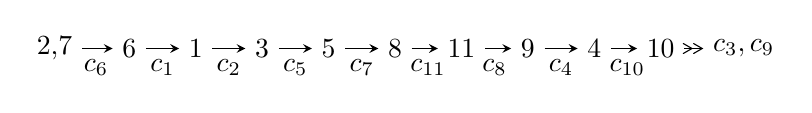
\begin{tikzpicture}[x=24pt, y=7pt]
	% node
	\node (A0) at (-1/8, 0) {2,7};
	\node (A1) at (1, 0) {6};
	\node (A2) at (2, 0) {1};
	\node (A3) at (3, 0) {3};
	\node (A4) at (4, 0) {5};
	\node (A5) at (5, 0) {8};
	\node (A6) at (6, 0) {11};
	\node (A7) at (7, 0) {9};
	\node (A8) at (8, 0) {4};
	\node (A9) at (9, 0) {10};
	\node (C1) at (1/2, -1) {$c_{6}$};
	\node (C2) at (3/2, -1) {$c_{1}$};
	\node (C3) at (5/2, -1) {$c_{2}$};
	\node (C4) at (7/2, -1) {$c_{5}$};
	\node (C5) at (9/2, -1) {$c_{7}$};
	\node (C6) at (11/2, -1) {$c_{11}$};
	\node (C7) at (13/2, -1) {$c_{8}$};
	\node (C8) at (15/2, -1) {$c_{4}$};
	\node (C9) at (17/2, -1) {$c_{10}$};
	\node (A10) at (41/4, 0) {$c_{3},c_{9}$};

	% edge
	\draw[->,>=stealth]	
	(A0) edge (A1) (A1) edge (A2) (A2) edge (A3) (A3) edge (A4) (A4) edge (A5) (A5) edge (A6) (A6) edge (A7) (A7) edge (A8) (A8) edge (A9) ;
	\draw[->>,>={angle 60}]	
	(A9) edge (A10);
\end{tikzpicture} \\ 

\end{tabular} \\

\footnotetext{
The image of knot diagram is generated by the software ``\textbf{Draw programme}" developed by Andrew Bartholomew(\url{http://www.layer8.co.uk/maths/draw/index.htm\#Running-draw}), where we modified some parts for our purpose(\url{https://github.com/CATsTAILs/LinksPainter}).
}\phantom \\ \newline 
\centering \textbf{Ideals for irreducible components\footnotemark of $X_{\text{par}}$} 
 
\begin{align*}
I^u_{1}&=\langle 
u^{35}- u^{34}+\cdots- u^2+1\rangle \\
\\
\end{align*}
\raggedright * 1 irreducible components of $\dim_{\mathbb{C}}=0$, with total 35 representations.\\
\footnotetext{All coefficients of polynomials are rational numbers. But the coefficients are sometimes approximated in decimal forms when there is not enough margin.}
\newpage
\renewcommand{\arraystretch}{1}
\centering \section*{I. $I^u_{1}= \langle u^{35}- u^{34}+\cdots- u^2+1 \rangle$}
\flushleft \textbf{(i) Arc colorings}\\
\begin{tabular}{m{7pt} m{180pt} m{7pt} m{180pt} }
\flushright $a_{2}=$&$\begin{pmatrix}0\\u\end{pmatrix}$ \\
\flushright $a_{7}=$&$\begin{pmatrix}1\\0\end{pmatrix}$ \\
\flushright $a_{6}=$&$\begin{pmatrix}1\\- u^2\end{pmatrix}$ \\
\flushright $a_{1}=$&$\begin{pmatrix}u\\- u^3+u\end{pmatrix}$ \\
\flushright $a_{3}=$&$\begin{pmatrix}- u^3\\u^5- u^3+u\end{pmatrix}$ \\
\flushright $a_{5}=$&$\begin{pmatrix}- u^2+1\\- u^2\end{pmatrix}$ \\
\flushright $a_{8}=$&$\begin{pmatrix}u^4- u^2+1\\u^4\end{pmatrix}$ \\
\flushright $a_{11}=$&$\begin{pmatrix}u^{11}-2 u^9+4 u^7-4 u^5+3 u^3\\u^{11}- u^9+2 u^7- u^5- u^3+u\end{pmatrix}$ \\
\flushright $a_{9}=$&$\begin{pmatrix}u^{18}-3 u^{16}+8 u^{14}-13 u^{12}+17 u^{10}-15 u^8+10 u^6-2 u^4- u^2+1\\u^{18}-2 u^{16}+5 u^{14}-6 u^{12}+5 u^{10}-2 u^8-2 u^6+4 u^4- u^2\end{pmatrix}$ \\
\flushright $a_{4}=$&$\begin{pmatrix}- u^{34}+5 u^{32}+\cdots- u^2+1\\- u^{34}+4 u^{32}+\cdots+4 u^6- u^2\end{pmatrix}$ \\
\flushright $a_{10}=$&$\begin{pmatrix}u^{19}-2 u^{17}+6 u^{15}-8 u^{13}+11 u^{11}-10 u^9+8 u^7-4 u^5+3 u^3\\- u^{21}+3 u^{19}+\cdots- u^3+u\end{pmatrix}$\\ \flushright $a_{10}=$&$\begin{pmatrix}u^{19}-2 u^{17}+6 u^{15}-8 u^{13}+11 u^{11}-10 u^9+8 u^7-4 u^5+3 u^3\\- u^{21}+3 u^{19}+\cdots- u^3+u\end{pmatrix}$\\&\end{tabular}
\flushleft \textbf{(ii) Obstruction class $= -1$}\\~\\
\flushleft \textbf{(iii) Cusp Shapes $= 4 u^{33}-4 u^{32}-16 u^{31}+20 u^{30}+64 u^{29}-76 u^{28}-160 u^{27}+204 u^{26}+356 u^{25}-440 u^{24}-624 u^{23}+772 u^{22}+948 u^{21}-1120 u^{20}-1204 u^{19}+1336 u^{18}+1308 u^{17}-1304 u^{16}-1180 u^{15}+984 u^{14}+888 u^{13}-528 u^{12}-512 u^{11}+128 u^{10}+216 u^9+80 u^8-40 u^7-96 u^6-16 u^5+32 u^4+16 u^3+4 u-10$}\\~\\
\newpage\renewcommand{\arraystretch}{1}
\flushleft \textbf{(iv) u-Polynomials at the component}\newline \\
\begin{tabular}{m{50pt}|m{274pt}}
Crossings & \hspace{64pt}u-Polynomials at each crossing \\
\hline $$\begin{aligned}c_{1},c_{6}\end{aligned}$$&$\begin{aligned}
&u^{35}- u^{34}+\cdots- u^2+1
\end{aligned}$\\
\hline $$\begin{aligned}c_{2},c_{5},c_{7}\end{aligned}$$&$\begin{aligned}
&u^{35}+9 u^{34}+\cdots+2 u+1
\end{aligned}$\\
\hline $$\begin{aligned}c_{3},c_{4},c_{9}\\c_{10}\end{aligned}$$&$\begin{aligned}
&u^{35}- u^{34}+\cdots+2 u+1
\end{aligned}$\\
\hline $$\begin{aligned}c_{8},c_{11}\end{aligned}$$&$\begin{aligned}
&u^{35}+7 u^{34}+\cdots+8 u+1
\end{aligned}$\\
\hline
\end{tabular}\\~\\
\newpage\renewcommand{\arraystretch}{1}
\flushleft \textbf{(v) Riley Polynomials at the component}\newline \\
\begin{tabular}{m{50pt}|m{274pt}}
Crossings & \hspace{64pt}Riley Polynomials at each crossing \\
\hline $$\begin{aligned}c_{1},c_{6}\end{aligned}$$&$\begin{aligned}
&y^{35}-9 y^{34}+\cdots+2 y-1
\end{aligned}$\\
\hline $$\begin{aligned}c_{2},c_{5},c_{7}\end{aligned}$$&$\begin{aligned}
&y^{35}+35 y^{34}+\cdots+18 y-1
\end{aligned}$\\
\hline $$\begin{aligned}c_{3},c_{4},c_{9}\\c_{10}\end{aligned}$$&$\begin{aligned}
&y^{35}+39 y^{34}+\cdots+2 y-1
\end{aligned}$\\
\hline $$\begin{aligned}c_{8},c_{11}\end{aligned}$$&$\begin{aligned}
&y^{35}+15 y^{34}+\cdots-14 y-1
\end{aligned}$\\
\hline
\end{tabular}\\~\\
\newpage\flushleft \textbf{(vi) Complex Volumes and Cusp Shapes}
$$\begin{array}{c|c|c}  
\text{Solutions to }I^u_{1}& \I (\text{vol} + \sqrt{-1}CS) & \text{Cusp shape}\\
 \hline 
\begin{aligned}
u &= \phantom{-}0.962624 + 0.303218 I\end{aligned}
 & -3.18298 - 4.64820 I & -10.32267 + 8.03074 I \\ \hline\begin{aligned}
u &= \phantom{-}0.962624 - 0.303218 I\end{aligned}
 & -3.18298 + 4.64820 I & -10.32267 - 8.03074 I \\ \hline\begin{aligned}
u &= \phantom{-}0.966916 + 0.178086 I\end{aligned}
 & \phantom{-}2.77604 + 1.42603 I & -8.39342 + 0.40844 I \\ \hline\begin{aligned}
u &= \phantom{-}0.966916 - 0.178086 I\end{aligned}
 & \phantom{-}2.77604 - 1.42603 I & -8.39342 - 0.40844 I \\ \hline\begin{aligned}
u &= -0.949626 + 0.247846 I\end{aligned}
 & -3.51316 + 0.86929 I & -12.03394 - 0.57851 I \\ \hline\begin{aligned}
u &= -0.949626 - 0.247846 I\end{aligned}
 & -3.51316 - 0.86929 I & -12.03394 + 0.57851 I \\ \hline\begin{aligned}
u &= -0.982664 + 0.344890 I\end{aligned}
 & \phantom{-}3.73413 + 7.15489 I & -6.21404 - 6.89294 I \\ \hline\begin{aligned}
u &= -0.982664 - 0.344890 I\end{aligned}
 & \phantom{-}3.73413 - 7.15489 I & -6.21404 + 6.89294 I \\ \hline\begin{aligned}
u &= -0.625205 + 0.585600 I\end{aligned}
 & \phantom{-}8.06862 + 2.14485 I & \phantom{-}0.03823 - 3.39579 I \\ \hline\begin{aligned}
u &= -0.625205 - 0.585600 I\end{aligned}
 & \phantom{-}8.06862 - 2.14485 I & \phantom{-}0.03823 + 3.39579 I \\ \hline\begin{aligned}
u &= \phantom{-}0.826215 + 0.817094 I\end{aligned}
 & \phantom{-}3.13686 - 1.06908 I & -6.00348 + 2.72542 I \\ \hline\begin{aligned}
u &= \phantom{-}0.826215 - 0.817094 I\end{aligned}
 & \phantom{-}3.13686 + 1.06908 I & -6.00348 - 2.72542 I \\ \hline\begin{aligned}
u &= -0.899785 + 0.739431 I\end{aligned}
 & \phantom{-}7.92591 + 2.80573 I & -2.67118 - 2.92017 I \\ \hline\begin{aligned}
u &= -0.899785 - 0.739431 I\end{aligned}
 & \phantom{-}7.92591 - 2.80573 I & -2.67118 + 2.92017 I \\ \hline\begin{aligned}
u &= -0.815673 + 0.849045 I\end{aligned}
 & \phantom{-}4.17141 - 2.71608 I & -3.22921 + 3.46654 I \\ \hline\begin{aligned}
u &= -0.815673 - 0.849045 I\end{aligned}
 & \phantom{-}4.17141 + 2.71608 I & -3.22921 - 3.46654 I \\ \hline\begin{aligned}
u &= \phantom{-}0.815012 + 0.872021 I\end{aligned}
 & \phantom{-}11.60150 + 5.24626 I & -0.28520 - 2.12331 I \\ \hline\begin{aligned}
u &= \phantom{-}0.815012 - 0.872021 I\end{aligned}
 & \phantom{-}11.60150 - 5.24626 I & -0.28520 + 2.12331 I \\ \hline\begin{aligned}
u &= -0.895926 + 0.820169 I\end{aligned}
 & \phantom{-}7.25366 + 3.06074 I & \phantom{-}0.53879 - 2.89823 I \\ \hline\begin{aligned}
u &= -0.895926 - 0.820169 I\end{aligned}
 & \phantom{-}7.25366 - 3.06074 I & \phantom{-}0.53879 + 2.89823 I \\ \hline\begin{aligned}
u &= \phantom{-}0.950191 + 0.783875 I\end{aligned}
 & \phantom{-}2.75474 - 4.93362 I & -6.65730 + 2.46852 I \\ \hline\begin{aligned}
u &= \phantom{-}0.950191 - 0.783875 I\end{aligned}
 & \phantom{-}2.75474 + 4.93362 I & -6.65730 - 2.46852 I \\ \hline\begin{aligned}
u &= \phantom{-}0.909352 + 0.854322 I\end{aligned}
 & \phantom{-}15.6759 - 3.1687 I & \phantom{-}1.84371 + 2.55774 I \\ \hline\begin{aligned}
u &= \phantom{-}0.909352 - 0.854322 I\end{aligned}
 & \phantom{-}15.6759 + 3.1687 I & \phantom{-}1.84371 - 2.55774 I \\ \hline\begin{aligned}
u &= -0.968524 + 0.797329 I\end{aligned}
 & \phantom{-}3.69689 + 8.85353 I & -4.28524 - 8.34437 I \\ \hline\begin{aligned}
u &= -0.968524 - 0.797329 I\end{aligned}
 & \phantom{-}3.69689 - 8.85353 I & -4.28524 + 8.34437 I \\ \hline\begin{aligned}
u &= \phantom{-}0.979984 + 0.808991 I\end{aligned}
 & \phantom{-}11.0850 - 11.4893 I & -1.26828 + 6.96489 I \\ \hline\begin{aligned}
u &= \phantom{-}0.979984 - 0.808991 I\end{aligned}
 & \phantom{-}11.0850 + 11.4893 I & -1.26828 - 6.96489 I \\ \hline\begin{aligned}
u &= \phantom{-}0.616861 + 0.373834 I\end{aligned}
 & \phantom{-}0.93698 - 1.48910 I & -0.78415 + 6.55847 I \\ \hline\begin{aligned}
u &= \phantom{-}0.616861 - 0.373834 I\end{aligned}
 & \phantom{-}0.93698 + 1.48910 I & -0.78415 - 6.55847 I\\
 \hline 
 \end{array}$$\newpage$$\begin{array}{c|c|c}  
\text{Solutions to }I^u_{1}& \I (\text{vol} + \sqrt{-1}CS) & \text{Cusp shape}\\
 \hline 
\begin{aligned}
u &= -0.163878 + 0.627930 I\end{aligned}
 & \phantom{-}6.28325 - 3.67948 I & -0.34607 + 2.46375 I \\ \hline\begin{aligned}
u &= -0.163878 - 0.627930 I\end{aligned}
 & \phantom{-}6.28325 + 3.67948 I & -0.34607 - 2.46375 I \\ \hline\begin{aligned}
u &= -0.621610\phantom{ +0.000000I}\end{aligned}
 & -0.791732\phantom{ +0.000000I} & -13.6740\phantom{ +0.000000I} \\ \hline\begin{aligned}
u &= \phantom{-}0.084932 + 0.544457 I\end{aligned}
 & -0.58473 + 1.62274 I & -4.08967 - 4.27499 I \\ \hline\begin{aligned}
u &= \phantom{-}0.084932 - 0.544457 I\end{aligned}
 & -0.58473 - 1.62274 I & -4.08967 + 4.27499 I\\
 \hline 
 \end{array}$$\newpage
\newpage\renewcommand{\arraystretch}{1}
\centering \section*{ II. u-Polynomials}
\begin{tabular}{m{50pt}|m{274pt}}
Crossings & \hspace{64pt}u-Polynomials at each crossing \\
\hline $$\begin{aligned}c_{1},c_{6}\end{aligned}$$&$\begin{aligned}
&u^{35}- u^{34}+\cdots- u^2+1
\end{aligned}$\\
\hline $$\begin{aligned}c_{2},c_{5},c_{7}\end{aligned}$$&$\begin{aligned}
&u^{35}+9 u^{34}+\cdots+2 u+1
\end{aligned}$\\
\hline $$\begin{aligned}c_{3},c_{4},c_{9}\\c_{10}\end{aligned}$$&$\begin{aligned}
&u^{35}- u^{34}+\cdots+2 u+1
\end{aligned}$\\
\hline $$\begin{aligned}c_{8},c_{11}\end{aligned}$$&$\begin{aligned}
&u^{35}+7 u^{34}+\cdots+8 u+1
\end{aligned}$\\
\hline
\end{tabular}\newpage\renewcommand{\arraystretch}{1}
\centering \section*{ III. Riley Polynomials}
\begin{tabular}{m{50pt}|m{274pt}}
Crossings & \hspace{64pt}Riley Polynomials at each crossing \\
\hline $$\begin{aligned}c_{1},c_{6}\end{aligned}$$&$\begin{aligned}
&y^{35}-9 y^{34}+\cdots+2 y-1
\end{aligned}$\\
\hline $$\begin{aligned}c_{2},c_{5},c_{7}\end{aligned}$$&$\begin{aligned}
&y^{35}+35 y^{34}+\cdots+18 y-1
\end{aligned}$\\
\hline $$\begin{aligned}c_{3},c_{4},c_{9}\\c_{10}\end{aligned}$$&$\begin{aligned}
&y^{35}+39 y^{34}+\cdots+2 y-1
\end{aligned}$\\
\hline $$\begin{aligned}c_{8},c_{11}\end{aligned}$$&$\begin{aligned}
&y^{35}+15 y^{34}+\cdots-14 y-1
\end{aligned}$\\
\hline
\end{tabular}
\vskip 2pc
\end{document}